\documentclass{article}
\usepackage[utf8]{inputenc}
\usepackage{dirtree}
\usepackage{listings}
\usepackage{color}
\usepackage{fancyhdr}
\usepackage{amsmath}
\usepackage{graphicx}
\usepackage{csvsimple}
\usepackage{booktabs}
\usepackage{tabularx}
\usepackage[margin=0.8in]{geometry}
\usepackage{float}
\usepackage{subfig}
\usepackage{listings}
\usepackage{upgreek}
\usepackage[american]{circuitikz}
\usepackage[titletoc,title]{appendix}
\usepackage{amssymb}
\usepackage{physics}
\usepackage{array,etoolbox}

\preto\tabular{\setcounter{magicrownumbers}{0}}
\newcounter{magicrownumbers}
\newcommand\rownumber{\stepcounter{magicrownumbers}\arabic{magicrownumbers}}

\title{D0018 Project Report}
\author{Anders Dahl, naddah-5\\
William Wennerström, wenwil-5}
\date{\today}

\begin{document}

\maketitle
\newpage

\tableofcontents
\newpage

\section{Executive summary}
Picoshop will be a webshop focused on simplicity and ease of use for both customers and employees. A minimalistic web interface will ensure that the products that are sold comes first.

During development a demo instance of Picoshop will be deployed that sells pickles, \textit{the to-go-place for your pickle needs}.

Picoshop will have support for a simple cart for customers, product listings and search capabilities. Employees have a easy web interface for handling orders in the warehouse, and also an administration interface for adding new articles.

\section{User stories}
We expect our users to be split into three main categories. Admins, employees and customers. The customers will have the ability to add orders into the system and to cancel orders that they have entered. Additionally they will be able to monitor their orders, accessing information on its status, in processing, shipping, etc. 

The employees refer to warehouse and shipping employees and will have the ability to complete orders, monitor relevant orders, and cancel orders. Relevant orders are defined as orders being processed in the specific location. A warehouse employee in Luleå will not be able to see orders being processed in Stockholm for example. Completion of a order will update the system and the stock available in the web-shop. The cancellation of a order will require a statement as to why it was canceled. This can be a result of defective stock, orders being bounced, i.e. sent back on the return address, as well as other unforeseen circumstances.

The admin users will in short have access to the entire system. They will have root access and as such only sensitive data will be unavailable to them. This includes but is not limited to user passwords and credit card information. Which will be encrypted.
\newpage

\section{System architecture}
To build our database we will use Go programming language with libraries for MySQL and MySQL driver to integrate the database with the website. 

The website will be built using HTML, CSS as well as JavaScript. In order to provide security we will use HTTPS for transport security and Bcrypt for hashing sensitive user data.

Finally we will use MySQLWorkbench to provide a system overview.

\subsection{Project structure}
\begin{figure}[H]
    \centering
    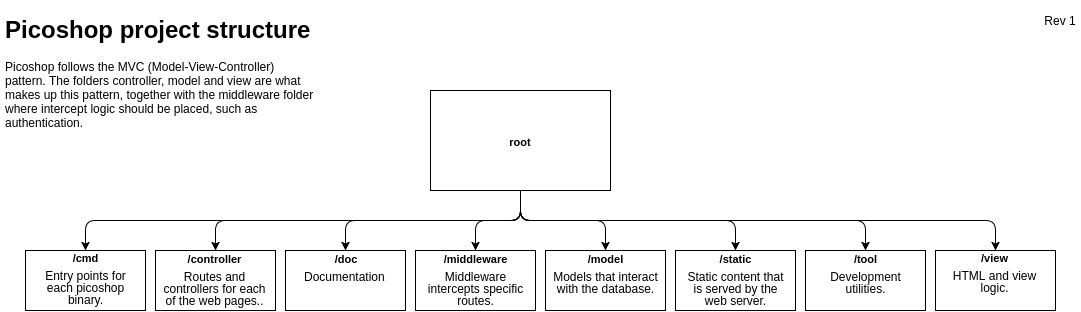
\includegraphics[width=17cm]{picoshop-project-structure_rev1.png}
    \caption{Internal code structure for Picoshop}
\end{figure}

\subsection{Web server API}
A web server API has been designed that follows the \emph{Representational state transfer} (REST) pattern. HTTP queries such as \texttt{/article/?id=\{id\}} is used instead of sub routes (\texttt{/article/\{id\}}) to simplify the implementation of routing and keeping the number of dependencies to a minimum, as per the Picoshop philosophy of minimalism. 
\begin{table}[H]
\centering
\caption{API endpoints and their methods}
\begin{tabular}{|clcl|}
\hline
\textbf{Method}              & \textbf{Endpoint}                             & \textbf{Access}              & \textbf{Description}                 \\ \hline
\multicolumn{1}{|c|}{GET}    & \multicolumn{1}{l|}{/}                        & \multicolumn{1}{c|}{N/A}     & Home page                            \\
\multicolumn{1}{|c|}{GET}    & \multicolumn{1}{l|}{/login}                   & \multicolumn{1}{c|}{N/A}     & View customer login page                      \\
\multicolumn{1}{|c|}{POST}   & \multicolumn{1}{l|}{/login}                   & \multicolumn{1}{c|}{N/A}     & Login customer user                           \\
\multicolumn{1}{|c|}{GET}    & \multicolumn{1}{l|}{/register}                & \multicolumn{1}{c|}{N/A}     & View customer register page                   \\
\multicolumn{1}{|c|}{POST}   & \multicolumn{1}{l|}{/register}                & \multicolumn{1}{c|}{N/A}     & Register customer user                        \\
\multicolumn{1}{|c|}{GET}    & \multicolumn{1}{l|}{/user}                    & \multicolumn{1}{c|}{C, W, A} & View user page                       \\
\multicolumn{1}{|c|}{POST}   & \multicolumn{1}{l|}{/user}                    & \multicolumn{1}{c|}{C, W, A} & Set user information                 \\
\multicolumn{1}{|c|}{GET}    & \multicolumn{1}{l|}{/article?id=\{0..n\}}     & \multicolumn{1}{c|}{C, W, A} & Get specific article by ID           \\
\multicolumn{1}{|c|}{POST}   & \multicolumn{1}{l|}{/cart}                    & \multicolumn{1}{c|}{C}       & Add artice to cart                   \\
\multicolumn{1}{|l|}{DELETE} & \multicolumn{1}{l|}{/cart?pos=\{0..n\}}       & \multicolumn{1}{c|}{C}       & Delete article from cart by position \\
\multicolumn{1}{|l|}{DELETE} & \multicolumn{1}{l|}{/cart}                    & \multicolumn{1}{c|}{C}       & Delete whole cart                    \\
\multicolumn{1}{|c|}{GET}    & \multicolumn{1}{l|}{/cart}                    & \multicolumn{1}{c|}{C}       & View cart                            \\
\multicolumn{1}{|c|}{PUT}    & \multicolumn{1}{l|}{/cart}                    & \multicolumn{1}{c|}{C}       & Order items in cart                  \\
\multicolumn{1}{|c|}{GET}    & \multicolumn{1}{l|}{/order}                   & \multicolumn{1}{c|}{W, A}    & View current orders                  \\
\multicolumn{1}{|c|}{GET}    & \multicolumn{1}{l|}{/order?id=\{0..n\}}       & \multicolumn{1}{c|}{W, A}    & View order by ID                     \\
\multicolumn{1}{|c|}{GET}    & \multicolumn{1}{l|}{/warehouse}               & \multicolumn{1}{c|}{W}       & Warehouse user home page             \\
\multicolumn{1}{|c|}{GET}    & \multicolumn{1}{l|}{/admin}                   & \multicolumn{1}{c|}{A}       & Admin user home page                 \\
\multicolumn{1}{|c|}{PUT}    & \multicolumn{1}{l|}{/order?id=\{0..n\}}       & \multicolumn{1}{c|}{W}       & Accept order by ID                   \\
\multicolumn{1}{|c|}{GET}    & \multicolumn{1}{l|}{/user?id=\{0..n\}}        & \multicolumn{1}{c|}{A}       & Display user by ID                   \\
\multicolumn{1}{|c|}{POST}   & \multicolumn{1}{l|}{/register?type=admin}     & \multicolumn{1}{c|}{A}       & Register new admin user              \\
\multicolumn{1}{|c|}{POST}   & \multicolumn{1}{l|}{/register?type=warehouse} & \multicolumn{1}{c|}{A}       & Register new warehouse user          \\
\multicolumn{1}{|c|}{POST}   & \multicolumn{1}{l|}{/register?type=customer}  & \multicolumn{1}{c|}{A}       & Register new customer user           \\ \hline
\end{tabular}
\end{table}

\subsection{Testing environment}
\subsubsection*{Backend}
A \emph{Continuous Integration} (CI) testing environment is used for unit testing. Travis CI Pro runs these tests on each new commit to the Git repository on GitHub. Go's built-in testing framework (\texttt{go test}) is used together with Bash and Dash shell scripts to run unit tests for the whole backend codebase.

\newpage
\section{Backlog}
For managing a live backlog the online tool ZenHub is used (see \url{https://www.zenhub.com}). Here is the latest snapshot of the backlog as of \today.

\subsection{Current overview}

\begin{table}[H]
\centering
\begin{tabular}{| @{\makebox[3em][c]{\rownumber.\space}} l|c|l|c|}
\multicolumn{4}{c}{\large{Sprint 1}} \\
\hline
\multicolumn{1}{|l}{\textbf{Title}} & \multicolumn{1}{l}{\textbf{Complexity}} & \multicolumn{1}{l|}{\textbf{Asignee}} & \multicolumn{1}{l|}{\textbf{Status}} \\ \hline 
Document changes in Sprint 1 & 21 & AD, WW & Done \\
Test suite for unit testing backend & 13 & WW & Done \\
Design web server API (routes/REST) & 8 & WW & Done \\
Implement initial HTML/CSS following design proposal & 21 & WW & Done \\
Connect database with web server & 5 & AD & Done \\
Implement initial web server following API proposal & 13 & WW & Done \\
First design proposal & 13 & AD & Done \\
Set up and test MySQL database & 8 & AD & Done \\
Create source code skeleton & 8 & WW & Done \\
Setup CI testing environment & 5 & WW & Done \\
\hline
\multicolumn{4}{r}{\textit{Due by: 2017-11-15}} \\

\multicolumn{4}{l}{} \\
\multicolumn{4}{c}{\large{Sprint 2}} \\
\hline
\multicolumn{1}{|l}{\textbf{Title}} & \multicolumn{1}{l}{\textbf{Complexity}} & \multicolumn{1}{l|}{\textbf{Asignee}} & \multicolumn{1}{l|}{\textbf{Status}} \\ \hline
Document changes in Sprint 2 & 21 & AD, WW & Backlog \\
Shopping cart support & 21 & WW & Backlog \\
Test suite for unit testing frontend & 21 & AD & Backlog \\
Login system (hashing + salting w/ Bcrypt) & 21 & AD & Backlog \\
Warehouse web interface & 21 & WW & Backlog \\
Admin web interface & 13 & AD & Backlog \\
Admin and Warehouse user login & 13 & WW & Backlog \\
Customer register and login & 13 & AD & Backlog \\
Customer-side order system & 40 & WW & Backlog \\
Finalize web interface design & 13 & AD & Backlog \\
Search support for articles & 21 & WW & Backlog \\
\hline
\multicolumn{4}{r}{\textit{Due by: 2017-11-30}} \\

\multicolumn{4}{l}{} \\
\multicolumn{4}{c}{\large{Sprint 3}} \\
\hline
\multicolumn{1}{|l}{\textbf{Title}} & \multicolumn{1}{l}{\textbf{Complexity}} & \multicolumn{1}{l|}{\textbf{Asignee}} & \multicolumn{1}{l|}{\textbf{Status}} \\ \hline
Load test of web interface & 21 & AD, WW & Backlog \\
Finalize GUI with improvements & 8 & WW & Backlog \\
Deploy application to server & 13 & AD & Backlog \\
Document changes in Sprint 3 & 21 & AD, WW & Backlog \\
Article grading support & 13 & WW & Backlog \\
Edit user profile & 13 & AD & Backlog \\
Article images & 8 & WW & Backlog \\
HTTPS/TLS support & 13 & WW & Backlog \\
Comment support for articles & 21 & AD & Backlog \\                         
\hline
\multicolumn{4}{r}{\textit{Due by: 2017-12-14}} \\

\end{tabular}
\end{table}

\subsection{Burndown reports}

\subsubsection*{Sprint 1}
\begin{figure}[H]
    \centering
    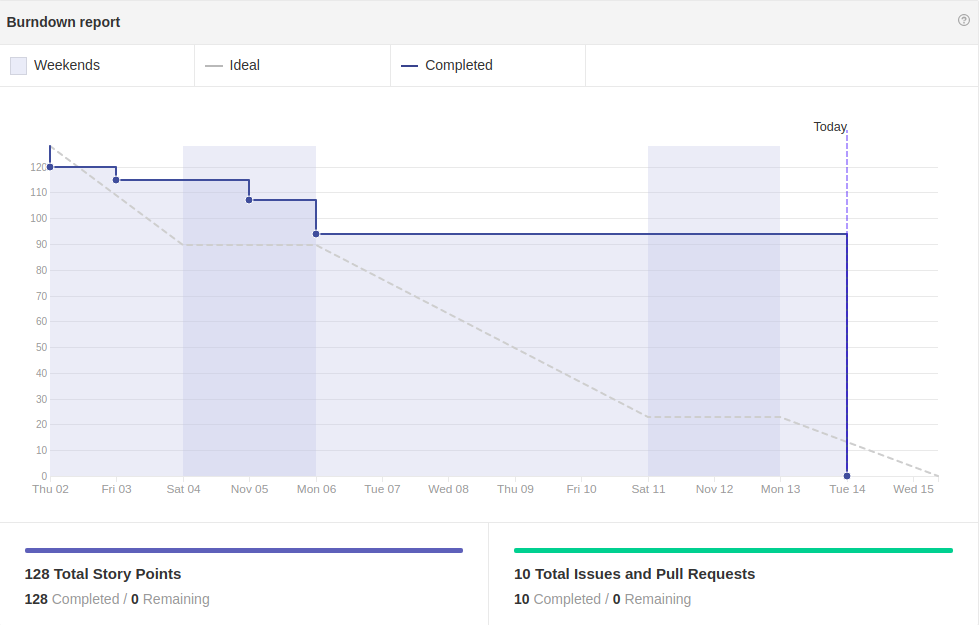
\includegraphics[width=17cm]{Burndown-report-1.png}
    \caption{Burndown report for Sprint 1}
\end{figure}

\section{Database schema}
\begin{figure}[H]
    \centering
    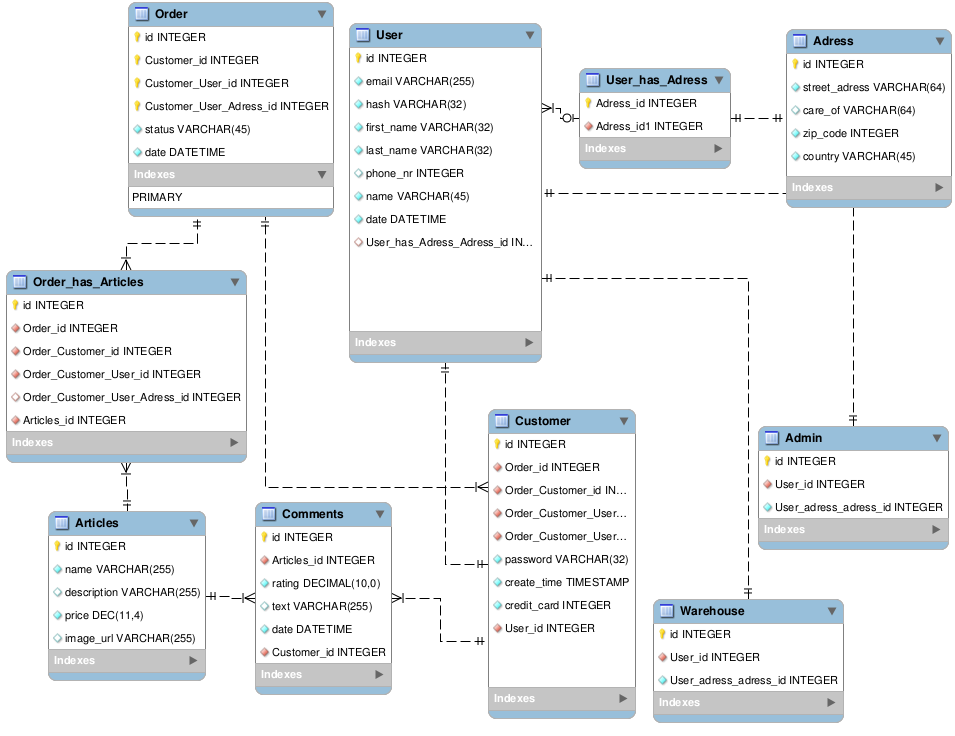
\includegraphics[width=16cm]{picoshop-sql-er-diagram-rev3.png}
    \caption{ER diagram for Picoshops SQL database}
    \label{fig:er-diagram}
\end{figure}

\newpage
\section{Test case specifications}

Currently there are no tests for the service. The tests will be documented according to the following template.

\bigskip
\hline
\subsection{Test case 1}
\subsubsection*{Purpose}
\subsubsection*{Requirement traceability}
\subsubsection*{Setup}
\subsubsection*{Test data}
\begin{table}[h]
\centering
\begin{tabular}{lll}
\hline
\multicolumn{1}{|l|}{\textbf{Action}} & \multicolumn{1}{l|}{\textbf{Input}} & \multicolumn{1}{l|}{\textbf{Output}} \\ \hline
& & \\
& & \\
& &                      
\end{tabular}
\end{table}
\subsubsection*{Notes}
\hline

\newpage
\section{System limitations and improvements}
The main limitations on the system will likely be multi-platform support. This however is a issue that is common to almost all websites and thus have solution patterns. Additional problems may arise as the project develop, such as multi-user compatibility and data security implementation. These issues will be solved by experimentation and practice. 

\section{Code and demo access}
\begin{table}[H]
\centering
\begin{tabular}{ll}
Git repository: & \href{git://github.com/willeponken/picoshop.git} \\
Git web interface: & \href{https://github.com/willeponken/picoshop} \\
Demo instance: & \textit{No instance is currently deployed.}
\end{tabular}
\end{table}

\end{document}
